\chapter{Methodology and Implementation}
\label{chap:metodology}

%goal 
Our goal with this project as outlined in \cref{chap:introduction} is creating a method for identifying LN relevant transactions on the blockchain and discover what information will be available to us by doing so. In \cref{sec:background} we covered how the LN uses the blockchain to operate, so the LN relevant transactions we are interested is the transactions in the blockchain used to operate LN channels. Because we are interested in what we can learn about the LN and its users from analyzing the blockchain, we will not utilize the information in non LN relevant transactions or users in this project. Reason behind this is the size of the blockchain as discussed in \cref{sec:related}, which means the requirements for both software and hardware will be high if all information should be kept track for parsing. The benefits of taking all information into consideration are also small four our project, however, it can be helpful and is discussed further in \cref{sec:future} on future work. 
\\

%blockchain vs ln
The link between the LN and the Bitcoin network will only provide us with a portion of the information about the LN and its users. By connecting to the LN itself we would have access to more information than found on the blockchain. However, the LN is a dynamic changing network of nodes, channels, and payment's; which is not stored in any public ledger like the blockchain. The information found in the LN can be recorded and stored by participants but the system itself does not keep such a record. The data in the blockchain can be verified by any user as explained in \cref{subsec:blockchain} while data recorded from the LN could not be verified in the same manner on its own.
This means that if we want historical data about the LN we must use the blockchain in which the users maintain a consensus about its correctness. Because as already stated the LN requires the Bitcoin system to operate so there will be on-chain transactions on the blockchain. We can also use the fact that there is much information available from connecting to the LN itself: collecting this information will allow us compare it with what we find on the blockchain. Doing this comparison we can verify our method for identifying LN relevant transactions on the blockchain. 
\\

\section{Blockchain analysis}
\label{sec:bc_analysis}

%subgraphs representing channels
The transactions in the blockchain is linked with outputs - inputs forming a DAG as we explained in \cref{subsec:transactions}. Parsing the blockchain would entail linking these transactions to form a transaction graph. When applying the heuristics used by previous works discussed in \cref{sec:background} one can use the information discovered there to provide context to the graph. In our work we do not create a complete transaction graph; we only link transactions related to a single LN channel which gives us a set of subgraphs of the complete transaction graph, each representing LN a channel. Only creating these small subgraphs is considerably easier because we do not need keep track as much data when the parsing is done. But to create these graphs we must first differentiate between on-chain LN transactions and normal Bitcoin transactions.
\\

%identifying, craeting subgraphs
To locate LN relevant transaction on the blockchain we identified attributes they contained not present in other transactions. As stated in \cref{subsec:pcln} Lightning channels have two main on-chain transactions: the founding/opening and closing transaction as seen in \cref{fig:ln_tx_graph} with the two middle transactions. The founding transaction will contain the channel output, and the closing transaction will have the channel input. This output - input pair will be of the type P2WSH 2of2 mutlsig as stated in \cref{subsec:pcln}. This will be the case for all output - input pairs used for these on-chain transactions, but it is not sufficient to determine if a transaction is related to the LN or not, because P2WSH 2of2 multisig transactions can be used for other purposes. As we explained in \cref{subsec:scripts} a P2SH (non segwit version of P2WSH) lock type will only have the hash of the script in the output, while the redeem script itself is included in the input of the spending transaction. This means that if we only consider a founding transaction output we will only be able to tell if the output is a P2WSH type, but if we only look at the closing tx input we will be able to tell that the type is P2WSH and that the redeem script is a 2of2 multisig script. Since both properties must be present in a LN channel output - input pair, we can say that it is more likely the transactions containing the inputs is relevant to LN based on the closing transaction rather than the founding tx. While this method cannot determine if transactions is related to the LN or not, it allows us to say that the transactions types in question are likelier than others to be LN related. We will discuss identification using this method later in this chapter.\todo{fix mutlisig}
\\

%timelocked tx
In addition to 2of2 multisig redeem scripts there is other script types used in certain LN on-chain transactions. One of these scripts is the one used when a channel is unilaterally closed-i.e., one of the parties in the channel publishes a commitment transaction. As explained in section \cref{subsec:pcln} the one who publishes a commitment transaction has their output of the commitment timelocked; this is to enable punishment for the publisher if the commitment in question was a revoked one with outdated balance favoring the publisher more than the most recent commitment. As stated in the LN specification \cite{bolt3} this unilaterally published commitment transaction has two outputs: one P2WPKH to the party who did not publish, and one P2WSH output with a redeem script which can be spent by waiting for the timelock it contains or with a revocation key. 
This redeem script is fairly unique and to our knowledge there is no other instances such scripts are used. However, people are free to create such scripts without it having anything to do with the LN, but the specific use case of such script makes this unlikely. Because the redeem script is located in the transaction spending a P2WSH output, we need for this case locate it in the transaction spending the timelocket output from the closing/commitment transaction. We will refer to this as the timelocked transaction which is shown on the right in \cref{fig:ln_tx_graph}. We explained in \cref{subsec:segwit} that each transaction has a id which is a hash of the transaction. This is how the transaction refer to each other; the inputs of transactions contain the transaction hash and output index of the transaction they spend. By looking for transactions with the redeem script for timelocked outputs we can identify the timelocked transactions, and because it will contain a reference to the transactions is spends we now also can locate the commitment/closing tx. Looking at the input to the commitment/closing transaction we can in turn find the founding tx. Doing this again with the founding transaction will give use the transactions used for input to the founding transaction. We are interested in these transactions which are used for input in the founding transaction for linking purposes which will be explained in \cref{sec:linking}. Using this method of first identifying the timelocked tx and then following the references to previous transactions found in the inputs will allow us to create subgraphs with transactions related to a LN channel as shown in \cref{fig:ln_tx_graph}.

\begin{figure}[h]
    \centering
    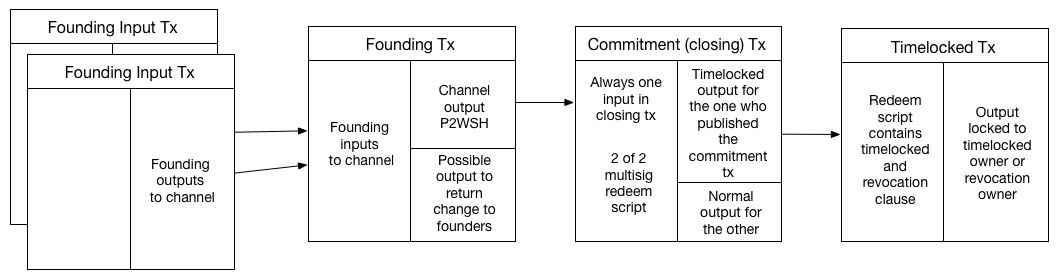
\includegraphics[width=14cm]{figures/ln_tx_graph.png}
    \caption{Transaction subgraph of unilaterally closed channel}
    \label{fig:ln_tx_graph}
\end{figure}


%% TODO closed channels only, add to ms detection potential p2wsh detection.
%reverse parsing
This method for locating subgraphs with LN related transactions is done in reverse when comparing to their creation time-i.e., we will find the timelocked transaction first and the tranactions used for input to the founding transaction last.
Because the tranasctions is a DAG as stated before, they will be located chronologically in the blockchain-e.g., the closing transactions cannot be found before the founding transaction as the closing uses the output of the founding.
We explained in \cref{subsec:blockchain} the blockchain confirms transactions and makes them valid by adding them to the chain; this means we must parse the blockchain in reverse order starting from the lastest block working our way down the the start. Doing this means we will encounter the relevant transactions in the order we want-i.e., for a subgraph we first encounter the timelocked tx and lastly the founding input transactions. We must also do this because the structure of the blockchain with blocks only referencing the previous one, only allowing us to traverse backwards in the chain. 
\\

%our software
In this project we have developed software parsing the blockchain and identified relevant transactions using the method outlined above.
We the btcd \cite{btcd_roasbeef} Bitcoin implementation for fetching and storing the blockchain data, and we also use libraries from it to read the data.
At a high level the software finds the top block from the blockchain data stored on disk and uses it as a starting point.
Then it traverses the transactions in the block and checks if they are relevant for our project, if that is the case they are stored for later use. After the transactions in a block is parsed the hash of the preceding block is used to get it from disk, and the same process is repeated.
Again, we create the LN channel transaction subgraph shown in \cref{fig:ln_tx_graph} by first looking for inputs containing the timelocked redeem script and then use the hash of the transaction that input spends to find the commitment/closing transaction.
The algorithm in its entirety is shown in \cref{fig:algo} where we the entire process of reading blocks and finding relevant transactions.
For each transaction we first check if it is a timelocked transaction, if it is we store as part of a subgraph for that channel and store the hash of the preceeding transaction (in this case the closing/commitment). As we parse tranasctions and identify tiemlocked transactions we have list of hashes known to be closing/commitment transaction, so if a transaction is not a timelocked one we check if the hash of the transaction matches any in the list. If it does we store it and finds the hash of the preceding (in this case the founding) and store it in a similar list; the same is done with founding input transactions. These hash lists are used to find all other transactions besides the timelocked in the subgraph. So for each transaction try to indeitfy it by checking if it is timelocked or the hash can be found in any of these lists. One thing to note is that a timelocked transaction can also be used as a input to a founding transaction, so we must also check found timelocked transaction against the list of founding input transactions; this will result in the same transaction being present in two subgraphs, with different role in each.

\begin{figure}[h]
    \centering
    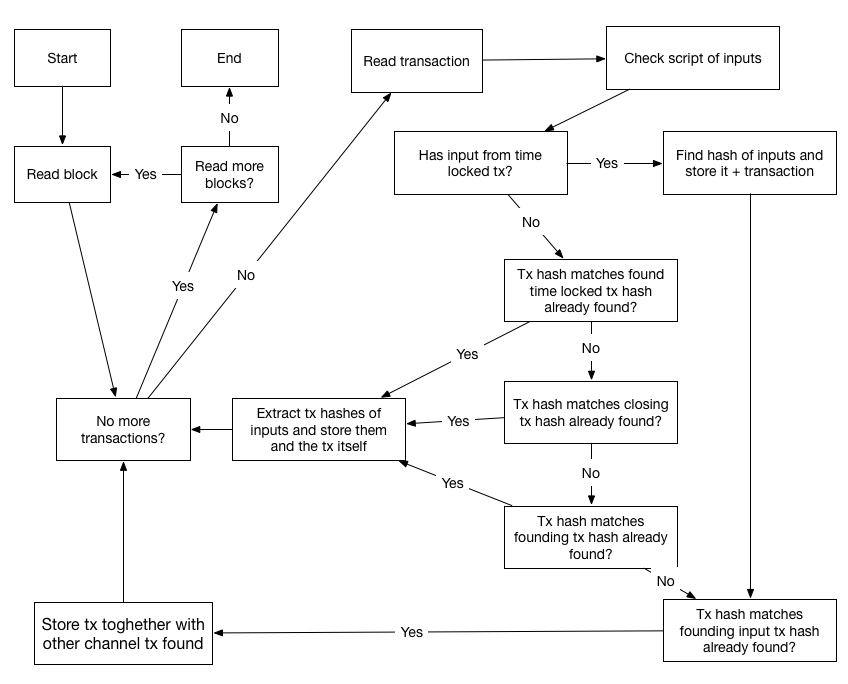
\includegraphics[width=14cm]{figures/algorithm.png}
    \caption{Algorithm of parsing and locating relevant LN transactions on the blockchain}
    \label{fig:algo}
\end{figure}


The redeem script used to identify the timelocked transactions is shown below: \cite{bolt3}
\\

\noindent OP\_IF \\
\indent   # Penalty transaction \\
\indent    <revocationpubkey> \\
OP\_ELSE\\
\indent    `to\_self\_delay`\\
\indent    OP\_CSV\\
\indent    OP\_DROP\\
\indent    <local\_delayedpubkey>\\
OP\_ENDIF\\
OP\_CHECKSIG\\

% timelocked script
The first line is the clause to stop participants from publishing old commitment transactions. The script will evaluate to true if this clause is used and the signature for the public key is given; As discussed in \cref{subsec:pcln} the parties will revoke old commitment transactions by exchanging keys so the other party can spend the timelocked output with the revocation key and get all the founds in the channel. The else clause is the timelocked portion of the script; it will contain a delay and the CHECKSEQUENCEVERIFY operation defined in \cite{BIP112} which terminates the script if the delay has not passed. The delay is then removed from the stack with OP\_DROP such that the signature and public key are the only two items on the stack when OP\_CHECKSIG is used to very the signature.
Our implementation takes the witness stack for each transaction it checks; see \cref{subsec:segwit} where we explained how the witness stack is structured for P2WSH transactions. Below we see the raw byte representation of the redeem script shown above. It has the same formatting and contains the same operations previously discussed as well as public keys and data.
%check segwit mandatory.
\\

\noindent [99 \\
\indent 33 3 251 83 243 198 231 109 204 252 217 94 44 221 0 255 185 86 106 105 161 141 254 96 
\indent 167 77 48 16 57 146 128 4 80 1 \\
103 \\
\indent 82 \\
\indent 178 \\
\indent 117 \\
\indent 33 2 159 6 236 212 233 63 48 147 59 52 201 11 15 138 165 248 118 100 188 234 227 215 
\indent 108 160 135 22 57 37 117 250 172 130 \\
104 \\
172]
\\

%byte rep of script
As we explained in \cref{subsec:scripts} the operations in the Bitcoin scripts is called opcodes, and the Bitcoin wiki contains a list of all of them with their encodings \cite{bitcoin_wiki_scripts}. These opcodes and their ordering in the script dictates the function of the script, so to identify this type of script we should look for scripts having the same format and operations.
The first byte vector seen in the raw script above is 99 which is the opcode for the the OP\_IF operation. The next vector is 33 which indicates how many bytes to push. 33 bytes is the length of a compressed public key with prefix. Bitcoin uses elliptic curve cryptography, where a public key is two coordinates representing a point on the curve. The prefix for compressed keys can be 02 or 03, and it indicates if the y coordinate is even or odd \cite{antonopoulos2017mastering}. So the third byte vector will always be 2 or 3, and the 32 next bytes will be the compressed key itself <revocationpubkey>. after the key we will find the OP\_ELSE with the opcode 103, followed by the 82 'to\_self\_delay' used for the OP\_CHECKSEQUENCEVERIFY (OP\_CSV) operation with opcode 178. Next vector is 117 which is the OP\_DROP 
operation. Next we have the <local\_delayedpubkey> in the same format as <revocationpubkey>, 33 is the bytes to push to the stak followed by the prefix and the compressed key itself. After that we have 104 which is the opcode for OP\_ENDIF, and 172 for OP\_CHECKSIG.
To identify redeem scripts from timelocked outputs of unilaterally closed lightning channels we check if the correct opcodes can be found at the exprected locations. E.g., index 0 of the script should be 99 for the OP\_IF, 103 for the OP\_ELSE should be at index 35 giving space for a public key. Each opcode used in the these type of scripts is used for recognition meaning the script must be a exact match to be identified as a timelocked redeem script.
\\

% multisig detection
The timelocked redeem scripts used to identify unilaterally closed channels are very unique compared to other scripts used, so when we find such scripts we can safely assume that the transaction is related to the LN. However, all channels cooperatively closed will not have the timelocked transaction shown in \cref{fig:ln_tx_graph} with the redeem script. They will instead only have a closing transaction outputting the balance to each party in the channel without any restrictions. Thus the subgraph showing all transactions related to a channel will be smaller and not contain the unique redeem script we previously have used. In the \cref{subsec:pcln} and the start of this section we discussed how the channel is built on a a P2WSH 2of2 multisig output located in the founding tx. We also mentioned that while this is not a unique characteristic of LN related transactions it can be used to rule out all transactions without this property.
If we use this method and rule out all transactions thats not of this type we will have the potentially LN relevant transactions left, determining how many of these is actually LN related is important as it will tell us how effective this method is. The effectiveness will depend on the use-cases for 2of2 multisig transactions and how widely it is currently used. E.g., if there is few uses beside LN channel transactions the method will be effective. We will try to determine the effectiveness of this method by comparing data from the blockchain with data gathered trough the LN. In \cref{sec:ln_analysis} we will discuss this more in detail, but the thinking is we will get the rate of actual LN relaed transaction from the potential set of LN transaction. 
\\

% how other information gathered. output types so on.
If we can successfully identify transaction subgraphs containing all transactions related to a LN channel we can use the data in those transactions to get some metrics about the channel. The value of the output - input pair used for the channel will tell us the total value of the channel. Timestamps is included in blocks when they are created, so by checking the timestamp of the blocks the founding and closing transactions is located in we can see how long the channel was operating. The number of inputs in the founding transactions and the number of outputs in the closing is also interesting; a founding transaction with a single input shows that a single user founded the channel; multiple inputs can indicate that both users founded the channel, but there is also a possibility that the channel is still founded by a single user, by using multiple smaller outputs to get the desired value of the channel. It is difficult to determine how founds have moved inside the channel based on value of the inputs to the founding transactions and the value of outputs from the closing transactions. Reason for this is that we normally cannot determine which input/output belong to which user in the channel. We discussed in \cref{subsec:scripts} on how keys are used to lock outputs and signatures is used in inputs to unlock, so a key pair is normally related to a input-output; we can see in \cref{fig:keys_subgraphs} a founding transaction with two inputs (keys), and a closing transaction with two outputs (keys). If we assume each user founded the channel with one input we can determine the initial balance by checking the value of those inputs. Comparing that balance to the one in the two outputs will tell us how it has shifted from start of the channel to the end. But as discussed in \cref{sec:related} the pseudonymity provided by new keys makes us unable to see which of the inputs corresponds to which output. We can also see in \cref{fig:keys_subgraphs} how the value is initially spread in two outputs then merged in the channel and then spread out again in two outputs, so simply following the specific value will not work. Linking the keys used in these transactions as done in previous work discussed in \cref{sec:related} will make this possible and is something we will discuess futher in \cref{sec:linking}. The one thing we can determine by looking at input, outputs of a channel is that a transaction has taken place in the channel, but this is only the case if there is one input to the funding transaction (single founded) and there is multiple outputs, so we know the channel started with with all value belonging to one party and it ends with the parties splitting the value.

\begin{figure}[h]
    \centering
    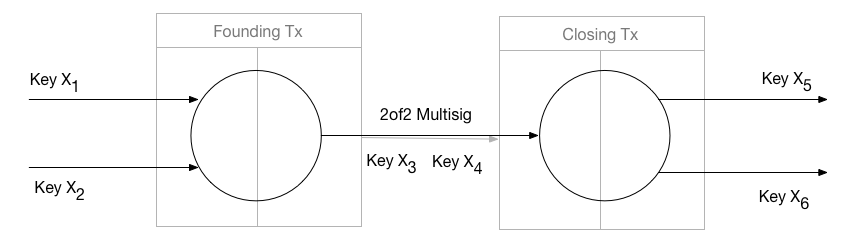
\includegraphics[width=14cm]{figures/keys_subgraph.png}
    \caption{Keys in transaction subgraph}
    \label{fig:keys_subgraphs}
\end{figure}

We can also get infomration about the LN by looking at transactions in general and not just channel subgraphs we have identified.
As we discussed earlier in this section the channel 2of2 multisig output - input is of the P2WSH type. Using this fact we can count the unspent P2WSH outputs and thus get the maximum upper limit of possible LN channels open. This can also be done to get the maximum number of channels at any historical point in the blockchain, by counting all P2WSH outputs and subtracting the spent ones up to a point on the blockchain will get us the unspent outputs at that point. While this will not accuratly show the number of channels (size) of the LN it will give us a concrete upper limit to its size.


\section{Lightning network analysis}
\label{sec:ln_analysis}

% lnd introduction
This project focuses on exploring the LN and related data trough the blockchain, but we can use other approaches verify and provide context to our methods and information. One such approach is simply to collect data from the LN directly. This data will be more complete than what we can find on the blockchain so it will provide us with the bigger picture. By comparing blockchain data with data directly from the LN, our methods of locating ln relevant data and their effectiveness can be measured. In \cref{sec:bc_analysis} we discussed using P2WSH (segwit) 2of2 multisig for detecting on-chain LN transactions, and we explained how we could measure the effectiveness of this method by comparing the results to known info from the LN. The data from the LN can also show relations between blockchain information we try to link, which will be explained in \cref{sec:linking}.
\\

To gather data from the LN we used a modified version of the LND implementation \cite{lnd}, which follows the BOLT specification \cite{bolt}. It maintains a view of the network by storing a graph containing active channels. This is continuously updated as new channels are announced trough the network, and closing transactions is found on new blocks on the blockchain. It requires a Bitcoin instance running to interact with the Bitcoin network; using it to publish on-chain transactions and monitor the blockchain. New channels are discovered by announcements within the LN while channels closing is found by looking at the blockchain and finding transactions spending the founding transactions of previously active channels. We forked and modified the LND deamon to create a copy of its database each time a new block notification was received from the Bitcoin software. This gave us snapshots of the Lightning Network every new block. 
\\

The snapshots contain a graph describing the state of the lightning network as known to our node at the time of the snapshot, so by comparing the graphs of different snapshots we can see how the network evolves over time. When comparing two snapshots from two points in time we can identify closed channels by checking the old snapshot for channels not found in the new one; Similarly new channels can be found by checking the new snapshot for channels not found in the old one. This allows us to build a list of channels closed and opened during the timeframe we collected data. 

% details getting channels.

% comparing to blockchain data

\section{Linking}
\label{sec:linking}
% intro clusting, goals and related work

Linking or clustering information that is related has been the focus of much of the related work described in \cref{sec:related}. The main goal there has been to construct user profiles by linking keys controlled by the same user. We are interested in the subset of Bitcoin users which is also LN users, in addition to the LN itself. 
Our method for discovering such information method have been outlined in \cref{sec:bc_analysis}, resulting in transaction subgraphs containing all transactions related to one channel. As we do not consider the entire Bitcoin transaction graph we cannot do a attempt a complete key linking for the entire blockchain, but we can link the channels represented by subgroups with each other.
As we know from \cref{subsec:networkpcln} the LN needs some nodes/users to have multiple channels such that a usable network is formed. Nodes in the LN can have many channels open, and channels will be related to each other by this fact. Any connection we can find in the two subgraphs will allow us to link the channels.
We are limited to linking metadata about the LN (channels/users/keys) as this is the information available on the blockchain; the channels is managed with these on-chain transaction, while transfers in this network will mostly be done off-chain.
\\

%defining a user
As stated we can link channels based on a common user participating on both, but we cannot determine which of the two users. 
The reason for this is the same as discussed in \cref{sec:bc_analysis} when we talked about matching inputs to outputs of a channel to see changes in balance between the users. 
In previous work discussed in \cref{sec:related} users where defined by control of a key pair, so essentially a key is a user.
Linking keys will reduce the number of users by redefining users as a set of key pairs.
Consider a transaction graph with four keys, there would be four potential users here unless we managed to link keys to reduce this.
In our case with the channel subgraphs, the problem arises because we know in advance how many users is involved in the transactions.
There is two users involved in a channel, but usually many more keys present, so we have a reduced user count but without linking any keys. Defining a user in this setting is harder, as we cannot simply choose a arbitrary key for each user. In \cref{fig:keys_subgraphs} we see how there is 6 keys which normally could each represent a user, but in our setting we know there is only two users. If we could link the keys and get two sets of keys belonging to each user, then this could be our definition of a user as it could be used to distinguish the users. 
\\

By linking channels based on shared user participation creates we can create a channel graph showing how the channels are related to each other. We can compare this to the transaction graph for Bitcoin which allows us to see how founds are moving by giving us the structure of the transaction graph, while the channel graph shows us how founds within the LN can move based on the structure of the network.
The LN is network itself, and therefore has a natural structure where nodes are users and the channels is edges between the users. This is a view which needs distinction between users, as each node in the network in is a single user (LN node). Transforming this graph to one where nodes represents channels and edges is a specific user participating in two channels, effectively connecting them. Such a channel centric view of the LN is similar to the one we attempted to make by linking channels, but the we can only link channels and not distinguish which user creates these connections.
\\

To create the channel graph we used three different heuristics for linking the channels. 
As mentioned any information found in the subgraphs relating it to another subgraph will allow us to link the two, illustrated in \cref{fig:linking_subgraphs}:

\begin{enumerate}
    \item \textbf{Key Reuse in different subgraphs} (red cirlce)\\
    The first heuristic is simply to check if the same keys has been reused in different channel subgraphs.  
A key found within a channel subgraph means it was involved with a LN channel, and if the same key can be found in more than one subgraphs we know the same user where involved in both.
This could be the key in any of the transactions found in the subgraph.
    
    \item \textbf{Output used in other Subgraph} (blue circle) \\
 The second heuristic is that subgraphs can be related based on outputs from transactions in one subgraph being used as inputs to transactions in another. The outputs is found in the founding, closing, or timelocked transaction; the input using such a output is found in the founding input transaction. This heuristic is the main reason we include this transaction in the channel subgraph. As these transactions provide the input to the founding transaction they are controlled by the participants in the channel, and therefore if they use a output from another channel we can determine the same user was present in both. As mentioned in \cref{sec:bc_analysis} the timelocked transaction in one subgraph can even be the founding input transaction in another, meaning the founding input can also provide overlap with the transaction graphs and not just a direct link with input - outputs.
    
    \item \textbf{Outputs from multiple subgrahps being inputs in one transaction} (green circle) \\
 The third heuristic is almost the same as the heuristic used by other projects discussed in \cref{sec:related} where keys was linked using multi-input transactions. 
 In our scenario with channel subgraphs we can do this check with the end outputs of the channel/subgraph-i.e., the output of the timelocked tx. If these outputs \todo{fix this}
    
\end{enumerate}

\begin{figure}[h]
    \centering
    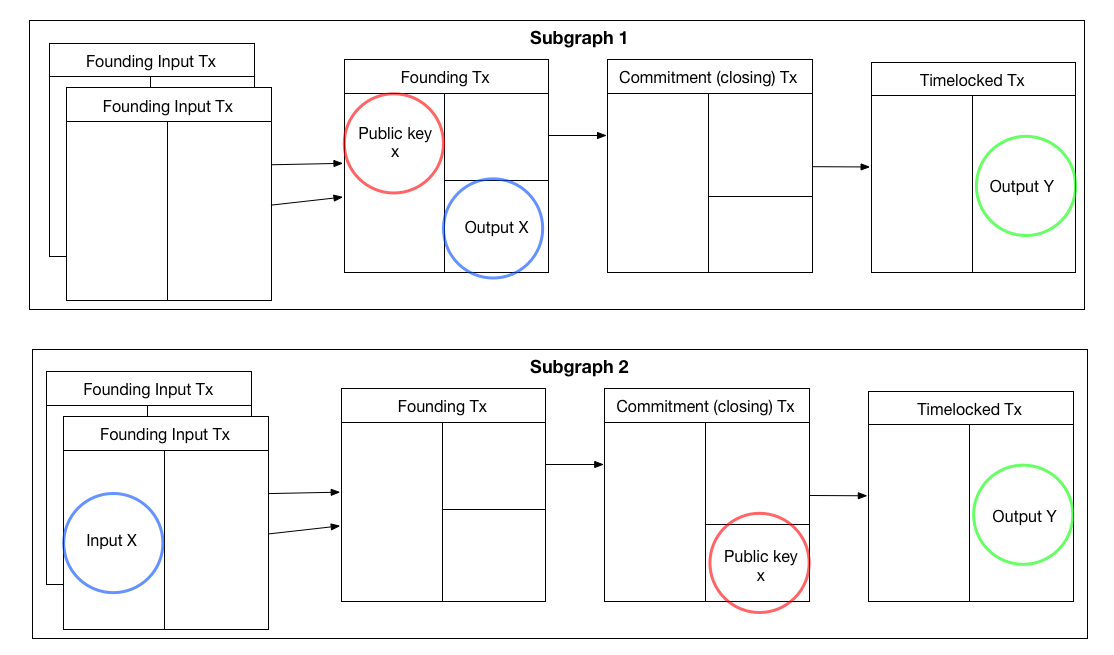
\includegraphics[width=14cm]{figures/linking_subgraphs.png}
    \caption{Methods for linking channels}
    \label{fig:linking_subgraphs}
\end{figure}

%todo, single founded tx, linking not possible if all founds tranasferred.

Defining a user when linking channels and using all information in the subgraph was problematic, but we can avoid this by only considering the keys in the 2of2 multisig output - input pair at the core of the channel subgraph. Using only these two keys will allow us  to differentiate the two users, and if any of the two keys is reused in other 2of2 multisig channel output - input pair we can determine which of the users is present in the other channel. Having clearly defined users we can identify in different channels would allow us to create a network where users is linked by participation in channels, similarly to the channel graph but here we can differentiate the users.
In such a network nodes would be users and edges channels between them, giving us the a network with a view like the standard LN view. However, when only considering this single output - input pair we have very little information to use for linking; we can not use the rest of the transactions in the subgraph as we run into the differentiating users problem again if we are unable to link the keys in the subgraph, so in our tests we have only done linking based on key reuse in the 2of2 multisig channel input - output. 